\documentclass[a4paper, 11pt]{article}
\usepackage[italian]{babel}
\usepackage[utf8x]{inputenc}
\usepackage[T1]{fontenc}
\usepackage{graphicx}
\usepackage{longtable}
\usepackage{float}
\usepackage{wrapfig}
\usepackage{rotating}
\usepackage[normalem]{ulem}
\usepackage{amsmath}
\usepackage{calc}
\usepackage{lastpage} % Required to determine the last page for the footer
\usepackage{extramarks} % Required for headers and footers
\usepackage{textcomp}
\usepackage{marvosym}
\usepackage{wasysym}
\usepackage{amssymb}
\usepackage{hyperref}
\usepackage{enumitem}
\usepackage[a4paper]{geometry}
\usepackage[section]{placeins}
\usepackage{lmodern}
%\usepackage[scaled=.85]{beramono}
\usepackage{array}
\usepackage{subcaption}
\usepackage{color}
\usepackage[usenames,dvipsnames,svgnames,table]{xcolor}
\usepackage{hyperref}
\hypersetup{
	colorlinks=true,
	linkcolor=black,
	urlcolor  = blue,
}
%\geometry{hmargin=2.3cm}

\topmargin=-0.45in
\evensidemargin=0in
\oddsidemargin=0in
\textwidth=6.25in
\textheight=9in
\headsep=0.25in

\usepackage[normalem]{ulem} % [normalem] prevents the package from changing the default behavior of `\emph` to underline.
\usepackage{fancyhdr}
\usepackage{array}

\renewcommand{\baselinestretch}{1.1} 

\newcommand{\hmwkTitle}{Med-H}

\pagestyle{fancy}
\lhead{\nouppercase{\leftmark}}
\rhead{\nouppercase{\rightmark}}
\chead{\hmwkTitle}
\lfoot{}
\cfoot{\thepage}
\rfoot{}
\renewcommand{\headrulewidth}{0.4pt}
\renewcommand{\footrulewidth}{0.4pt}


\def\changemargin#1#2{\list{}{\rightmargin#2\leftmargin#1}\item[]}
\let\endchangemargin=\endlist 

\newcolumntype{L}{>{\fontseries{l}\selectfont\arraybackslash}p{0.7\textwidth}}

\newcommand{\safeImage} [2] [\textwidth]{%
	\begin{figure}[H]
		\centering
	\IfFileExists{#2}{\includegraphics[width={#1},keepaspectratio]{#2}}{\includegraphics{example-image-a}}
	\end{figure}
}

\newcommand{\breakcell}[2][l]{\begin{tabular}[t]{@{}#1@{}}#2\end{tabular}}

\newcommand{\usecase}[5]{%
\begin{table}[H]
	%\vspace*{0.5 cm}
	\centering
	\renewcommand{\familydefault}{\ttdefault}\normalfont
\begin{tabular}{| >{\fontseries{b}\selectfont} p{0.2\textwidth} | L |}
	\hline
	ID&{#1}\\\hline
	Attori&{#2}\\\hline
	Precondizioni&{#3}\\\hline
	Sequenza&{#4}\\\hline
	Postcondizioni&{#5}\\\hline
\end{tabular}
\end{table}

}

\begin{document}

	\clearpage
%	\maketitle
\begin{titlepage}
	\centering
	\vspace*{\fill}
	
\includegraphics[width=0.15\textwidth]{logo.png}\par\vspace{1cm}
	{\scshape\LARGE Università degli Studi di Verona \par}
	\vspace{1cm}
	{\scshape\Large Ingegneria del Software\par}
	\vspace{1.5cm}
	\line(1,0){250} \\
	{\huge\bfseries Med-H\par}
	{\Large\bfseries Documentazione al prototipo\par}
	\line(1,0){250} \\
	\vspace{2cm}
	{\Large\itshape Mirko Morati, Noè Murr\par}
	\vspace{5cm}
	\vspace*{\fill}
	% Bottom of the page
	{\large \today\par}
\end{titlepage}
\thispagestyle{empty}
\newpage
\tableofcontents
\newpage

\section{Introduzione}
Obiettivo dell'elaborato è la progettazione di un prototipo software per la gestione delle prescrizioni di farmaci da parte dei medici di base di una regione.

In questa relazione ci proponiamo di raccogliere la documentazione sviluppata e di fornire spiegazioni e dettagli sulle scelte progettuali ed implementative. 

\section{Requisiti}
Di seguito viene riportato il testo dell'elaborato. I requisiti vengono identificati con una linea tratteggiata.

\begin{changemargin}{1cm}{0.5cm} 
Si vuole progettare un sistema informativo per gestire le prescrizioni di farmaci da parte dei medici di base di una regione. Il medico di base effettua la prescrizione di farmaci su richiesta del paziente (nel caso di farmaci legati a malattie croniche del paziente stesso) o in seguito alla visita. Nel caso di prescrizione su richiesta, il paziente può richiedere la prescrizione alla segreteria del medico che si occuperà di raccogliere le richieste, far preparare le ricette al medico e consegnare le prescrizioni ai pazienti.

\dashuline{I farmaci potranno essere prescritti anche da eventuali medici consorziati con il medico di base di riferimento o in caso di assenza del medico di base, dal medico sostituto designato}.
\dashuline{Ogni prescrizione è caratterizzata dall’indicazione del paziente a cui fa riferimento, dalla data di emissione, dalla data di scadenza, dai farmaci prescritti. Ogni prescrizione è dotata di un codice identificativo univoco}. La prescrizione deve essere presentata in farmacia per poter acquistare i farmaci necessari. Il farmacista utilizza la prescrizione, unitamente alla tessera sanitaria del paziente, per rilasciare lo scontrino parlante. In caso il medico abbia prescritto un farmaco e la farmacia non ne abbia a disposizione, il farmacista provvederà ad ordinare il farmaco per il paziente.
\dashuline{Per ogni paziente sono memorizzati: il codice sanitario univoco, il cognome, il nome, la data di nascita, il luogo di nascita, l’indirizzo di residenza (via, civico, cap, città, provincia). Per ogni paziente è possibile memorizzare gli eventuali fattori di rischio presenti (anche più d’uno)}.

\dashuline{Per ogni medico di base si registrano il codice fiscale, il codice univoco assegnato a livello regionale, il cognome, il nome, la data e il luogo di nascita. Per i medici di base con specializzazione si registrano anche l’ultima specializzazione ottenuta e la data di conseguimento. Ad ogni medico sono legate tutte le prescrizioni effettuate}.

\dashuline{Il medico può richiedere al sistema di visualizzare la lista dei farmaci prescritti ad un certo paziente in un certo periodo di tempo (mese, trimestre, semestre o anno)}, oppure \dashuline{la lista di farmaci prescritta nel complesso su base mensile o annuale}. Inoltre \dashuline{può verificare se e quando qualche paziente non ha usato la prescrizione emessa o se un paziente ha preferito il farmaco generico}.

\dashuline{In ogni prescrizione possono apparire al più 5 farmaci}. \dashuline{Ogni farmaco è caratterizzato da nome commerciale univoco, dal costo, dalla forma farmaceutica, dalle controindicazioni, e dalla sua classificazione secondo il sistema ATC (Anatomico-Terapeutico-Chimico)}. \dashuline{Per ogni farmaco si tiene traccia dei principi attivi contenuti: per ogni principio attivo di un farmaco sono indicati la quantità contenuta in ogni unità di farmaco (ad esempio, “500 mg per compressa” o “120 mg per ml”). Per ogni principio attivo sono memorizzati un nome univoco, una sua descrizione e l’effetto principale}. \dashuline{Il medico può poi specificare quali prescrizioni contengono farmaci che potrebbero interagire con risultati negativi per il paziente. In tal caso sono specificate le coppie di farmaci della stessa prescrizione che possono interagire}.

\dashuline{Il medico può richiedere al sistema di visualizzare la quantità di un certo farmaco prescritta ai suoi pazienti su base mensile, trimestrale, semestrale o annuale}. \dashuline{Può anche visualizzare la lista dei pazienti a cui ha prescritto un certo farmaco} e la lista delle eventuali reazione avverse comunicate all'agenzia di riferimento.
\end{changemargin}

\section{UML}
In questa sezione sono presentati i diagrammi richiesti per la documentazione del prototipo. 

\subsection{Use Cases}
% Sequence diagram per i principali use cases insieme alle schede
Gli use case individuati sono stati suddivisi in due macroaree definite dalla scelta di disposizione della GUI:

\begin{enumerate}[nosep] 
	\item Vista con focus sui pazienti
	\item Vista con focus sui farmaci.
\end{enumerate}

Di seguito vengono proposte alcune schede descrittive degli use case principali.

\safeImage[0.7\textwidth]{Vista_paziente.png}

\safeImage[0.7\textwidth]{Vista_farmaci.png}

\usecase{UC1: Inserimento paziente.}
{Medico}
{Il medico deve aver effettuato il login.}
{%
	\begin{enumerate}[label*=\arabic*., nosep]
		\item Il medico preme il pulsante di aggiunta paziente e viene visualizzato il dialog corrispondente.
		\item Inserisce i dati relativi alla persona ed eventuali fattori di rischio.
		\item Se il medico preme Ok:
		\begin{enumerate}[label*=\arabic*., nosep]
			\item Viene effettuata la validazione dei dati immessi. Se sono validi:
			\begin{enumerate}[label*=\arabic*., nosep]
				\item Il paziente viene inserito a database.
				\item Il dialog viene chiuso.
			\end{enumerate}
			Se non sono validi viene visualizzato un messaggio di errore.
		\end{enumerate}
		\item Se il medico preme Annulla:
		\begin{enumerate}[label*=\arabic*., nosep]
			\item Il dialog viene chiuso.
		\end{enumerate}
	\end{enumerate}}
{La lista dei pazienti è aggiornata.}

\usecase{UC2: Inserimento prescrizione.}
{Medico}
{Il medico deve aver effettuato il login.}
{%
	\begin{enumerate}[label*=\arabic*., nosep]
		\item Il medico seleziona un paziente.
		\item Il medico preme il pulsante di aggiunta prescrizione e viene visualizzato il dialog corrispondente.
		\item Inserisce i dettagli della prescrizione.
		\item Se il medico preme Ok:
		\begin{enumerate}[label*=\arabic*., nosep]
			\item Viene effettuata la validazione dei dati immessi. Se sono validi:
			\begin{enumerate}[label*=\arabic*., nosep]
				\item La prescrizione viene aggiunta al database.
				\item Il dialog viene chiuso.
			\end{enumerate}
			Se non sono validi viene visualizzato un messaggio di errore.
		\end{enumerate}
		\item Se il medico preme Annulla:
		\begin{enumerate}[label*=\arabic*., nosep]
			\item Il dialog viene chiuso.
		\end{enumerate}
\end{enumerate}}
{La lista delle prescrizioni è aggiornata.}

Il seguente use case è stato pensato per soddisfare il requisito della visualizzazione della lista dei farmaci prescritti ad un certo paziente in un certo periodo di tempo.
\usecase{UC3: Visualizza prescrizioni di un paziente.}
{Medico}
{Il medico deve aver effettuato il login.}
{
	\begin{enumerate}[label*=\arabic*., nosep]
		\item Il medico deve selezionare un paziente.
		\item Il medico può applicare un filtro:
		\begin{enumerate}[label*=\arabic*., nosep]
			\item Il filtro viene attivato.
			\item Viene selezionato un range tra mese, trimestre, semestre, anno e custom.
			\item Viene selezionata una data di inizio per modificare il range.
		\end{enumerate}
\end{enumerate}
}
{La lista delle prescrizioni è aggiornata.}


\usecase{UC4: Visualizza pazienti a cui è stato prescritto il farmaco.}
{Medico}
{Il medico deve aver effettuato il login.}
{\begin{enumerate}[label*=\arabic*., nosep]
		\item Il medico deve selezionare un farmaco.
		\item Il medico può applicare un filtro:
		\begin{enumerate}[label*=\arabic*., nosep]
			\item Il filtro viene attivato.
			\item Viene selezionato un range tra mese o anno.
			\item Viene selezionata una data di inizio per modificare il range.
		\end{enumerate}
\end{enumerate}}
{La lista dei pazienti è aggiornata.}

\usecase{UC5: Visualizza quantità di farmaco totale prescritta.}
{Medico}
{Il medico deve aver effettuato il login.}
{\begin{enumerate}[label*=\arabic*., nosep]
		\item Il medico deve selezionare un farmaco.
		\item Il medico può modificare il filtro relativo alla quantità:
		\begin{enumerate}[label*=\arabic*., nosep]
			\item Viene selezionato un range tra mese, trimestre, semestre e anno.
			\item Viene selezionata una data di inizio per modificare il range.
		\end{enumerate}
\end{enumerate}}
{La label della quantità è aggiornata.}

\newpage
\subsection{Activity Diagram}
I seguenti activity diagram cercano di modellare in modo più dettagliato il flusso d'esecuzione relativo ad alcuni degli use case precedentemente proposti. 
Si noti che i diagrammi relativi agli use case \texttt{UC4} e \texttt{UC5} risulterebbero molto simili al diagramma presentato per lo use case \texttt{UC3}.

\safeImage{Inserimento_paziente.png}
\safeImage{Inserimento_prescrizione.png}
\safeImage{Visualizza_farmaci_per_paziente.png}

\newpage
\subsection{Class Diagram}
Il class diagram qui proposto non è comprensivo di attributi e proprietà, serve a dare un'idea generale dell'organizzazione del prototipo software.
Si rimanda al class diagram completo all'Appendice A.
\begin{figure}[H]
	\centering
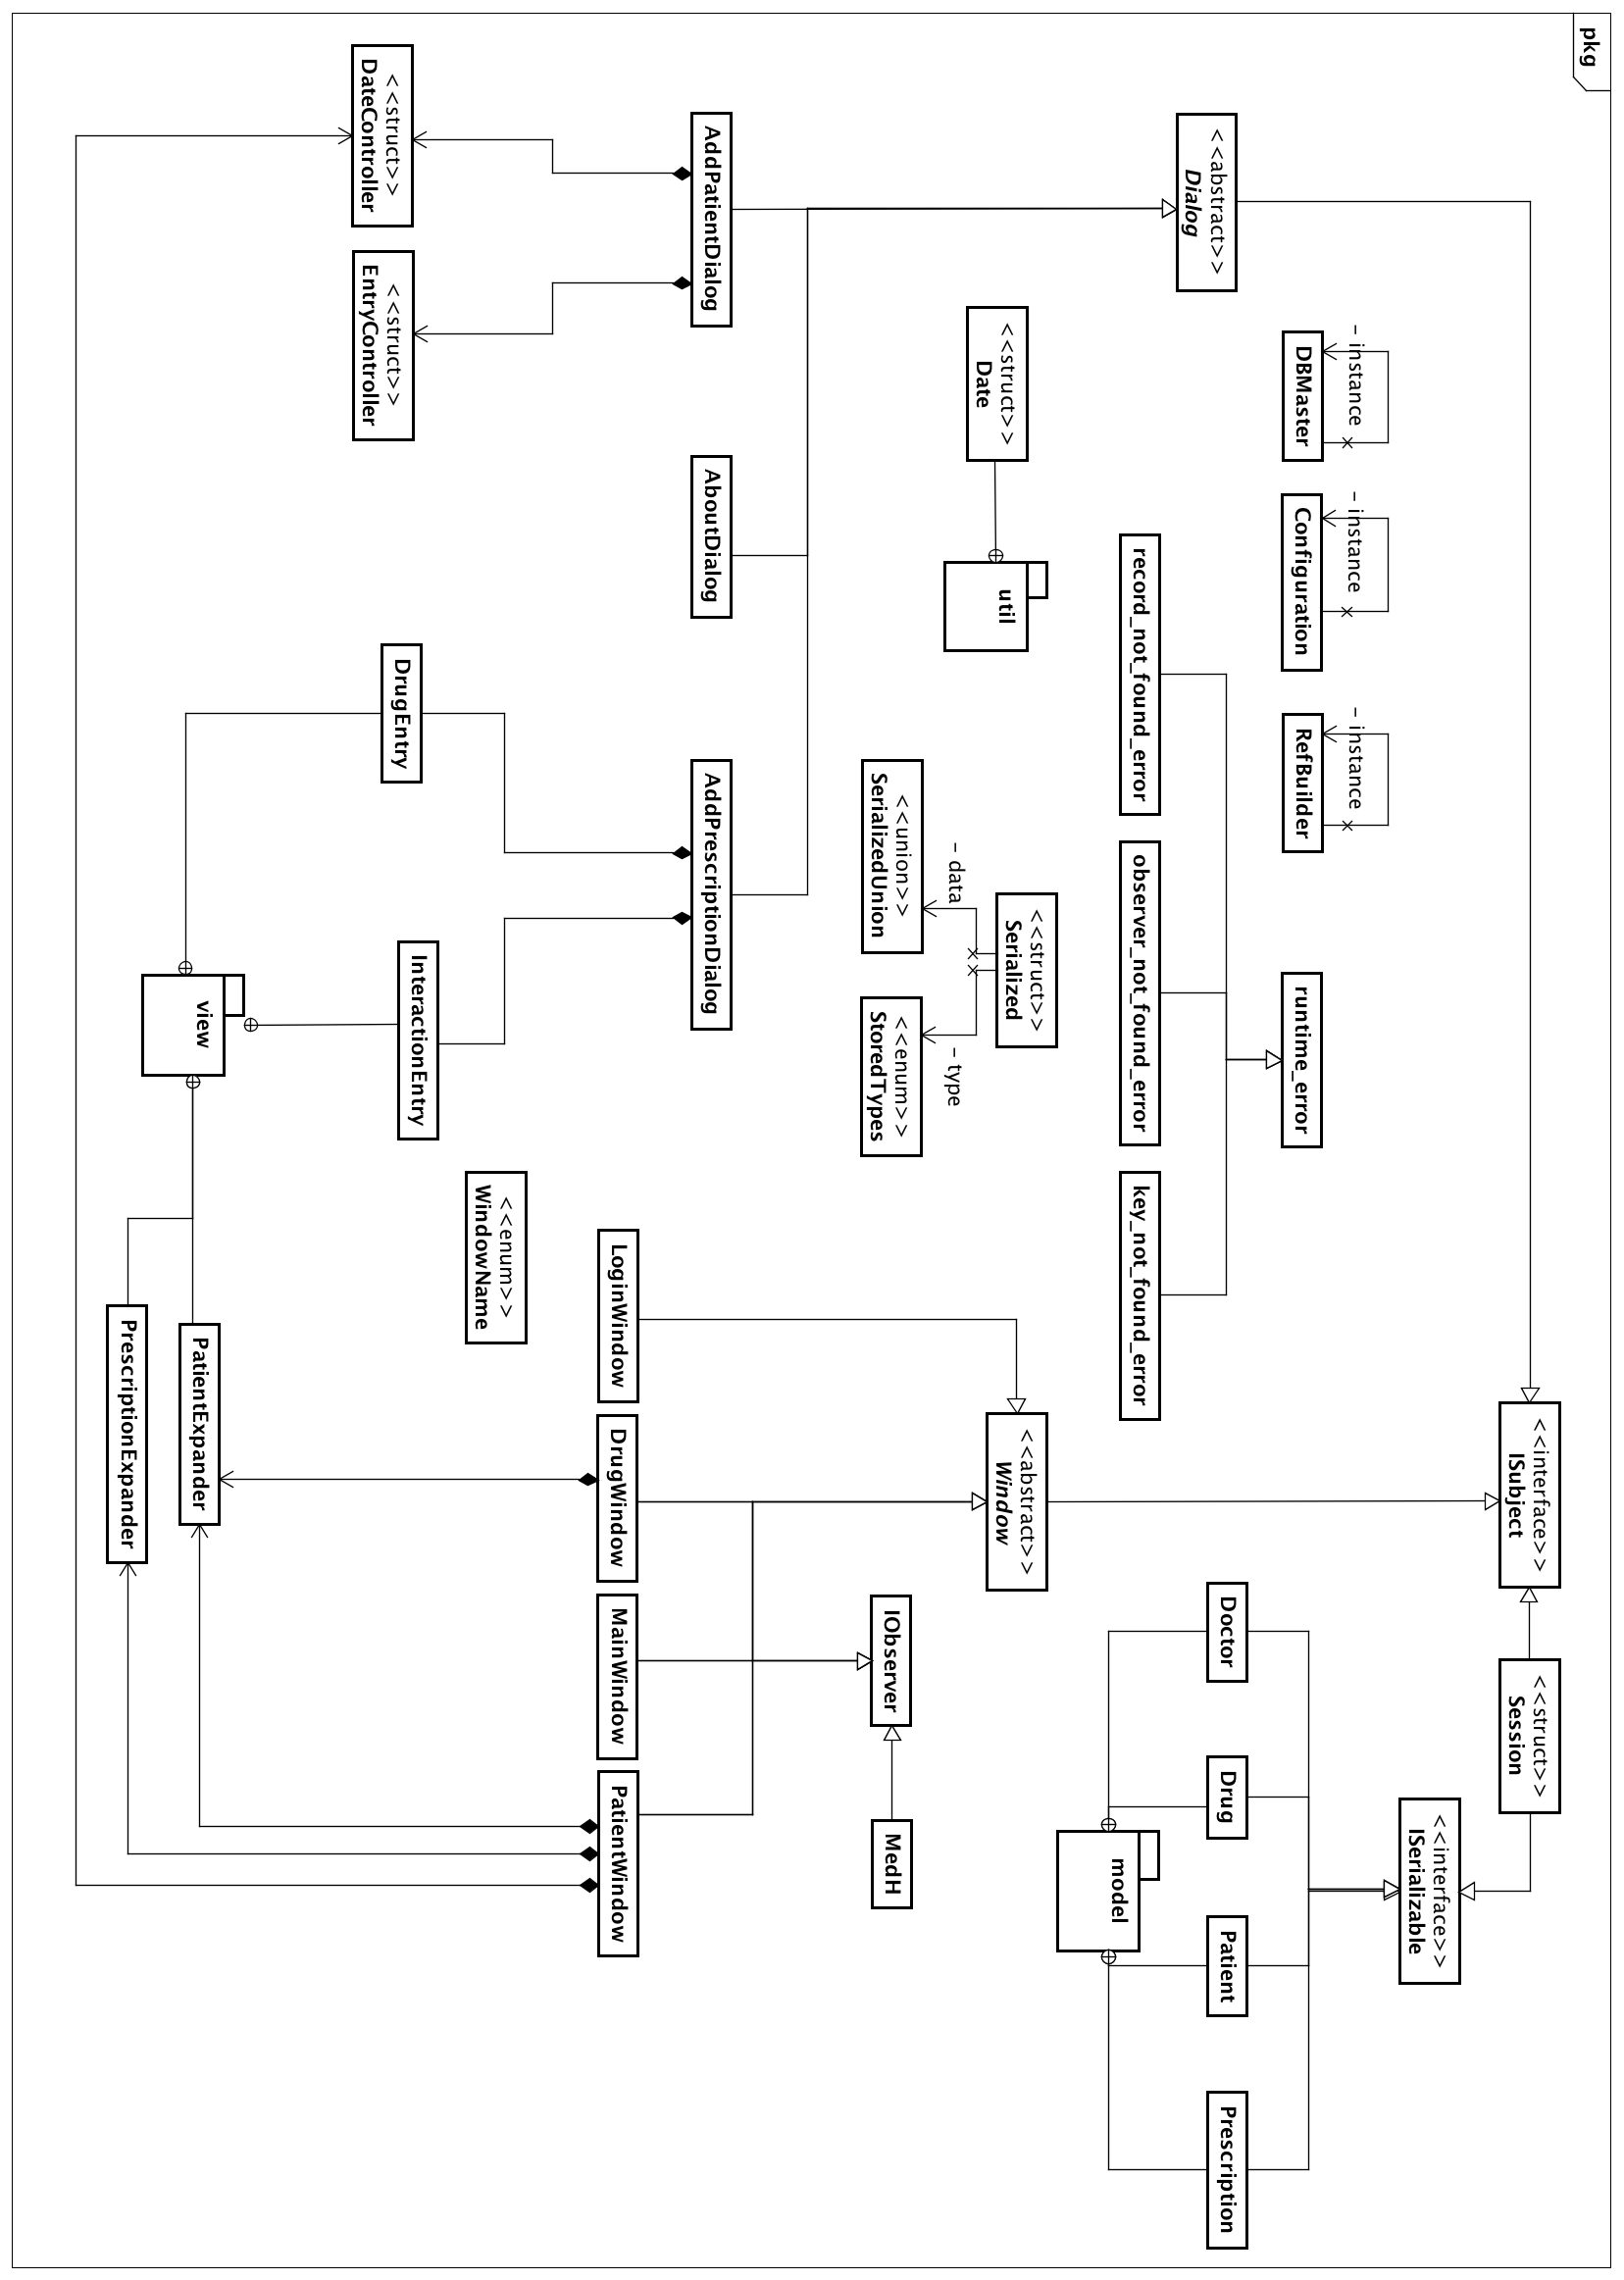
\includegraphics[width=0.9\textwidth,keepaspectratio]{Class_diagram_min.png}
\end{figure}

\newpage
\subsection{Sequence Diagram}
\safeImage{Inserimento_paziente_seq.png}
\safeImage{Visualizza_prescrizioni_filtrate_seq.png}
\safeImage{Login_sequence_seq.png}

\section{Scelte Progettuali}
\subsection{Sviluppo}
Abbiamo scelto di sviluppare il prototipo usando il linguaggio C++ in modo da poter ampliare la nostra conoscenza applicando i nuovi standard ad un progetto reale.
L'obbligo di rispettare dei requisiti applicando dei pattern di programmazione orientata agli oggetti ci ha spinti a ricercare ed implementare soluzioni al di fuori della nostra esperienza.

Uno stimolo in più l'abbiamo ricevuto quando abbiamo deciso di usare la libreria grafica Gtkmm3, un'interfaccia verso la più popolare libreria Gtk+. Alcune delle feature che ci hanno spinto ad operare questa scelta sono state:
\begin{itemize}[nosep]
	\item uso dell'ereditarietà per definire nuovi widget
	\item type-safe signal handlers
	\item polimorfismo
	\item management automatico della memoria in C++
	\item cross-platform
	\item open source
\end{itemize}

Oltre a questo abbiamo trovato utile la possibilità di costruire la GUI utilizzando il RAD tool Glade, un designer di interfacce grafiche.
La definizione dell'interfaccia risiede in un file XML che viene parsato all'inizio del programma ed i widget costruiti vengono resi disponibili tramite una classe singleton (si veda MVC Pattern). 
Da notare il supporto completo dei componenti agli stili CSS: la libreria non esclude la possibilità di personalizzare l'interfaccia senza passare dal tool né la creazione di temi da parte di utenti.

\subsubsection{Metodologia di Sviluppo}
Il progetto è stato interamente sviluppato usando Git come sistema di versionamento del codice e Github per l'hosting del repository.
Abbiamo seguito una metodologia di sviluppo Agile: dopo aver analizzato i requisiti del testo proposto abbiamo diviso il lavoro in due macroaree (logica ed user interface).
Le aree sono state suddivise in task brevi e di facile implementazione, testando gradualmente il nuovo codice inserito. I design pattern applicati sono stati decisi nella fase di sviluppo valutando di volta in volta le necessità per mantenere il progetto leggibile e scalabile. 

In molte occasioni è stato necessario operare un refactoring del codice per migliorare in efficacia il prototipo. Il sistema di versionamento ci ha permesso di dividere logicamente i task in branch e mantenere una cronologia delle modifiche in modo da poterle eventualmente scartare.

\subsection{Database}
Siccome si è reso necessario mantenere un insieme di dati persistenti abbiamo deciso di appoggiarci al sistema di database Sqlite3. Purtroppo le nostre competenze in basi di dati all'inizio del progetto erano alquanto scarne, quindi più che essere utilizzato come un vero e proprio RDBMS è stato utilizzato quasi come se i dati fossero organizzati in file.

È stata realizzata una classe di interfacciamento che provvede a nascondere la complessità delle transazioni (si veda Facade Pattern).

\subsection{Organizzazione della GUI}
È possibile individuare tre sezioni principali della GUI del prototipo, ognuna delle quali cerca di rispondere ad un insieme di requisiti specifici:
\begin{enumerate}[label=(\alph*)., nosep]
	\item Login: permette l'autenticazione del medico, prerequisito fondamentale per tutti gli use case definiti. 
	\item Tab pazienti: il focus è sui pazienti legati al medico autenticato. In questa sezione è possibile vedere, filtrare ed aggiungere le prescrizioni relative ad un paziente (oltre ad altre operazioni), in questo modo è possibile vedere l'elenco di farmaci prescritti ad un paziente in un dato periodo.
	\item Tab farmaci: il focus è sui farmaci disponibili a database. In questa sezione è possibile per ogni farmaco visualizzare, in un determinato periodo, una lista dei pazienti a cui è stato prescritto con dettagli. È anche possibile visualizzare la quantità di un determinato farmaco prescritta a tutti i pazienti in un determinato periodo. 
\end{enumerate}

\begin{figure}[H]
	\begin{subfigure}[t]{\textwidth}
		\centering
		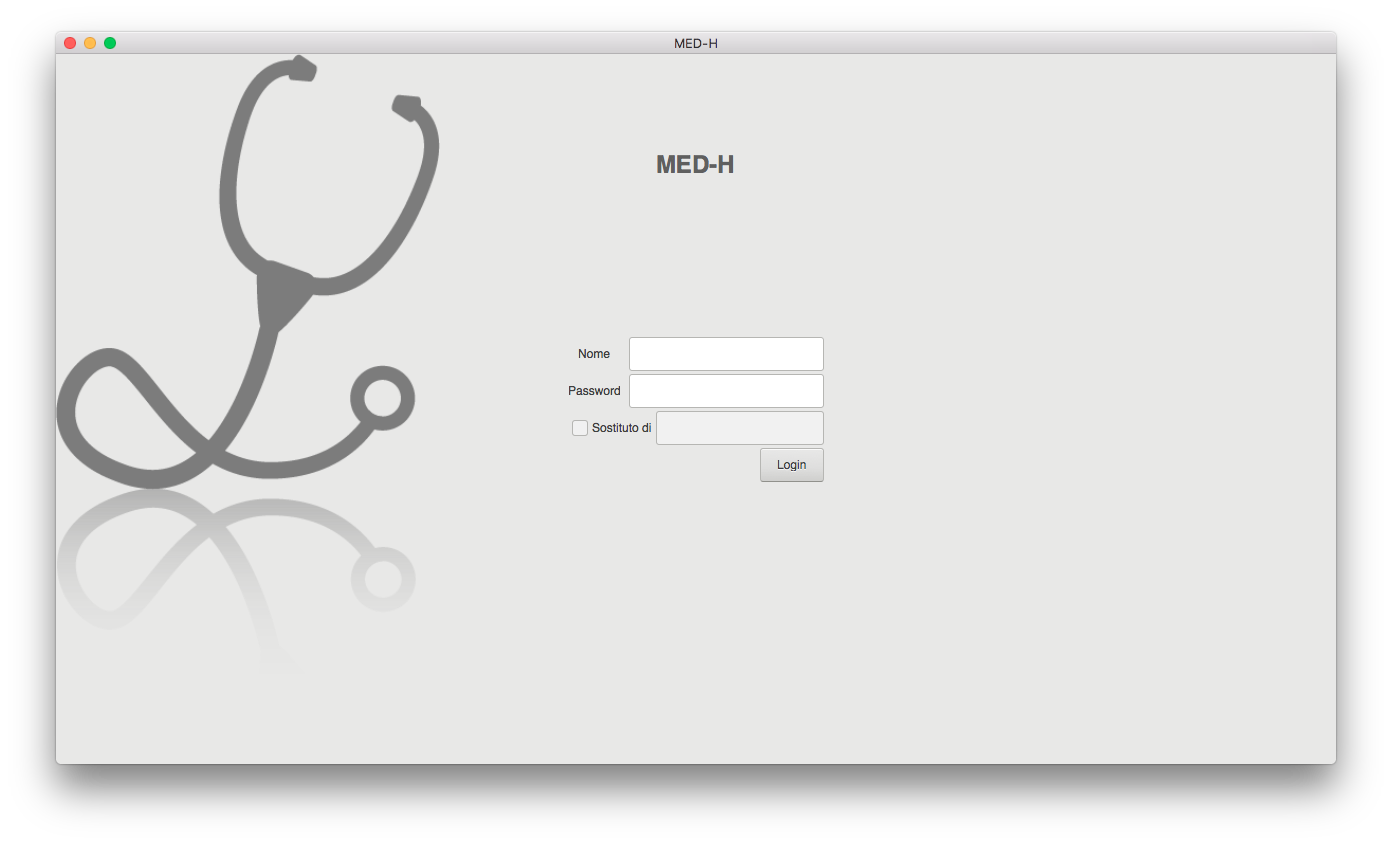
\includegraphics[height=0.3\textheight]{login}
		\caption{Schermata di Login}
	\end{subfigure}
\begin{subfigure}[b]{\textwidth}
	\centering
	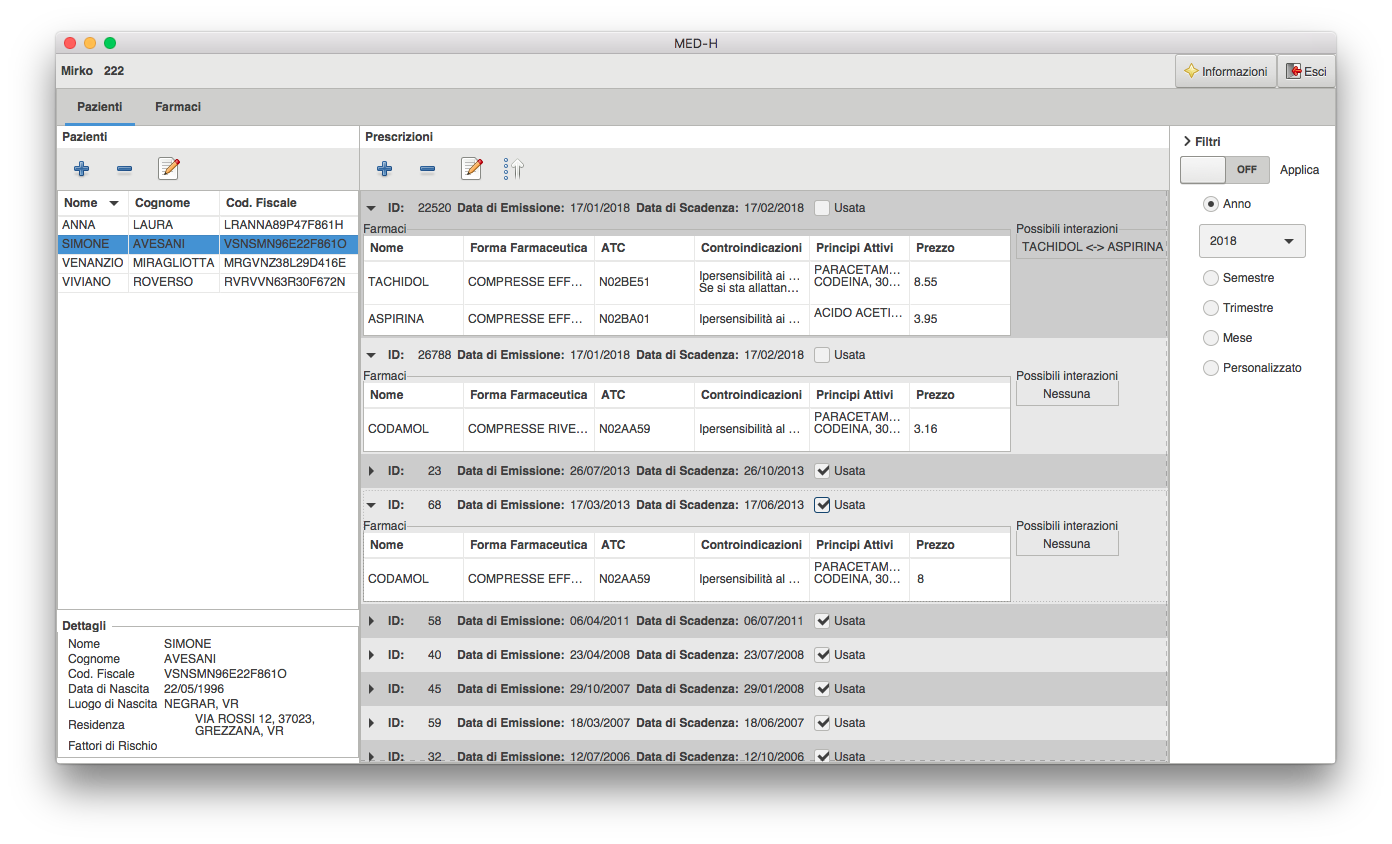
\includegraphics[height=0.3\textheight]{pazienti}
	\caption{Tab Pazienti}
\end{subfigure}
\begin{subfigure}[b]{\textwidth}
	\centering
	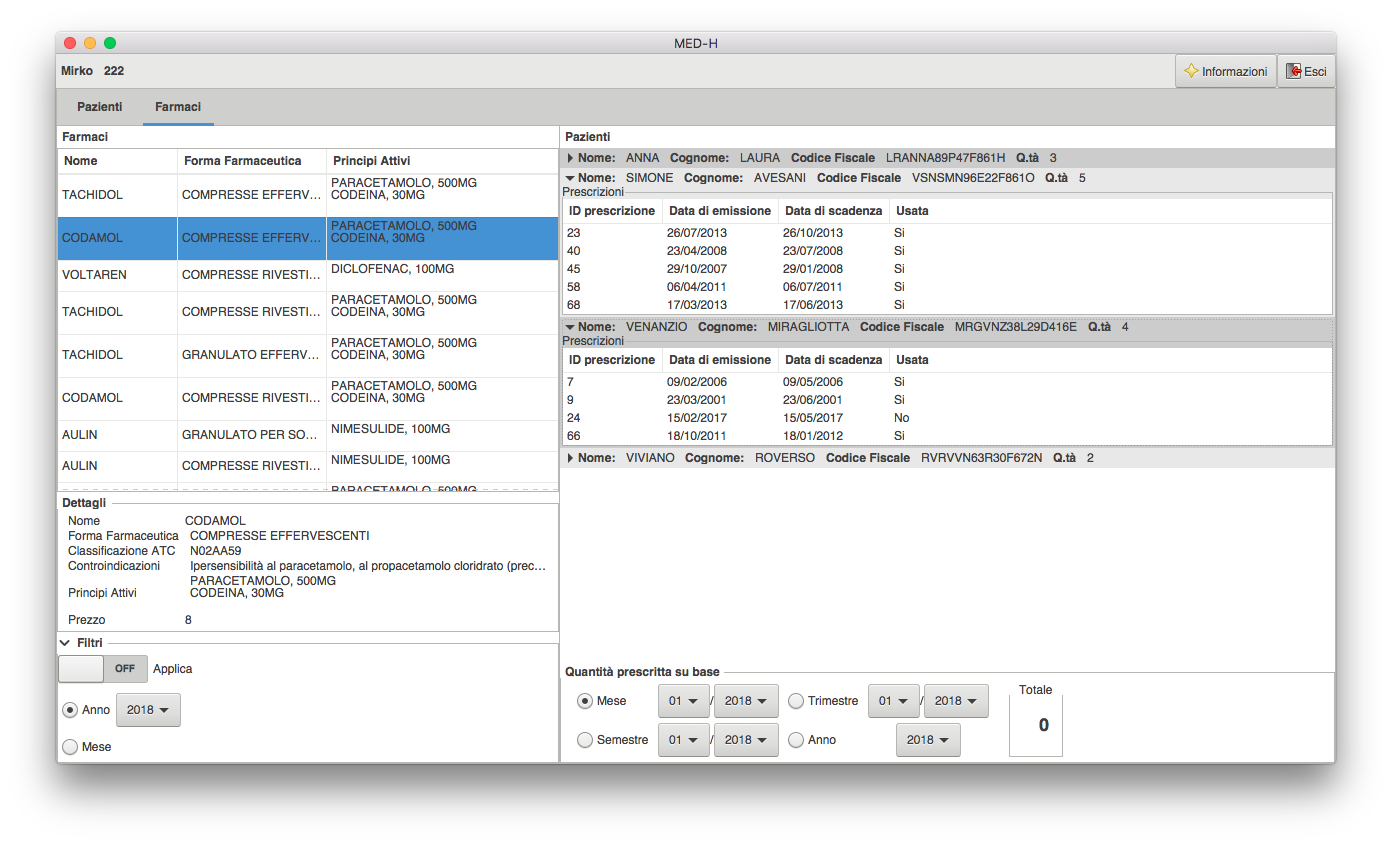
\includegraphics[height=0.3\textheight]{farmaci}
	\caption{Tab Farmaci}
\end{subfigure}
\end{figure}

\subsection{MVC Pattern}
L'applicazione del pattern prevede la suddivisione logica delle classi in tre componenti: model, view, controller. 
Abbiamo adattato il pattern per poterlo sfruttare al meglio nonostante la realizzazione dell'interfaccia grafica in XML abbia reso complicato organizzare la comunicazione tra view e relativi controller.
La libreria Gtkmm3 mette a disposizione un Builder che si occupa della costruzione della view a partire dall'XML; per rendere disponibili i widget ai controller abbiamo realizzato un singleton che si occupa di fornire un'interfaccia di collegamento.

Svantaggio di questa soluzione è la mancanza di un incapsulamento reale che impedisca ad un controller di accedere ad un widget di una view con cui non dovrebbe avere collegamenti. Questo è un compito lasciato al programmatore.

\safeImage[0.7\textwidth]{mvc.png}

\subsection{Singleton Pattern}
Per raccogliere insiemi di funzioni che necessitavano di una configurazione, abbiamo ottenuto opportuno utilizzare il singleton pattern. In questo modo abbiamo fornito in tutto il codice la possibilità di utilizzare un insieme di interfacce inizializzate in un punto solo del programma (e "safe").
Le classi che adottano il pattern sono: 

\begin{itemize}[nosep]
	\item DBMaster
	\item RefBuilder
	\item Configuration
	\item Login.
\end{itemize}

Da notare che in C++ è possibile definire due implementazioni differenti per il singleton pattern, una lazy e una eager. La nostra implementazione è lazy, ovvero l'istanza della classe viene creata solo alla prima richiesta di utilizzo.

\subsection{Observer Pattern}
Anche l'observer pattern è stato adattato al prototipo. Viene utilizzato per sincronizzare i dialog con le rispettive view principali in caso di modifiche che rendono necessario un aggiornamento. 

A differenza del pattern originale la nostra implementazione permette di specificare un parametro nella notifica in modo da poter differenziare gli update in ogni observer.
Nel prototipo non si è reso necessario (ma rimane possibile) specificare più di un observer per ogni subject. 

\subsection{Facade Pattern}
Il facade pattern permette di ``mascherare'' per mezzo di un'interfaccia di semplice utilizzo la complessità di un'operazione. È stato adottato nella classe DBMaster per fornire dei metodi che coprano l'utilizzo della libreria (sviluppata in C) per l'accesso al database sqlite.

\section{Validazione}
La parte di codice ritenuta più critica è quella relativa alle transazioni a database. Abbiamo scritto degli unit test utilizzando la libreria open source Catch2 che permette di creare test case in modo semplice e veloce. 

Per quanto riguarda l'interfaccia utente abbiamo dovuto testarla manualmente in quanto non abbiamo trovato un metodo automatico. È stato anche richiesto ad alcuni colleghi di provare il prodotto in modo da raccogliere feedback sull'esperienza di utilizzo dello stesso.

\section{Conclusioni}
Obiettivo del progetto non era quello di sviluppare un prodotto finito e completo ma di realizzare un prototipo rispettando le linee guida. Per questo non sono state implementate alcune funzionalità e l'interfaccia è rimasta ``grezza''. 
Al termine del progetto abbiamo convenuto che la scelta della libreria per l'interfaccia grafica non è stata delle più ottimali poiché purtroppo la documentazione manca di validi esempi e non è sempre intuitivo passare dall'idea al codice.

Il progetto completo può essere trovato alla pagina di \href{https://github.com/mirkomorati/elaborato_ING_SW}{Github}.

\end{document}
